\documentclass{article}
\usepackage[utf8]{inputenc}
\usepackage[brazilian]{babel}
\usepackage{geometry}
\geometry{a4paper, total={150mm,240mm}, top=25mm}
\usepackage{graphicx}
\usepackage{titling}
\usepackage{float}

\title{Exercício Prático 1 - Círculo Mínimo}
\author{Kleyton da Costa (2312730)}
\date{\today}
 
\usepackage{fancyhdr}
\fancypagestyle{plain}{%  the preset of fancyhdr 
    \fancyhf{} % clear all header and footer fields
    \fancyfoot[R]{
\includegraphics[width=3cm]{di.png}}
    \fancyfoot[L]{\today}
    \fancyhead[L]{Geometria Computacional}
    \fancyhead[R]{\theauthor}
}
\makeatletter
\def\@maketitle{%
  \newpage
  \null
  \vskip 1em%
  \begin{center}%
  \let \footnote \thanks
    {\LARGE \@title \par}%
    \vskip 1em%
    %{\large \@date}%
  \end{center}%
  \par
  \vskip 1em}
\makeatother

\begin{document}

\maketitle

\noindent\begin{tabular}{@{}ll}
    Aluno & \theauthor \\
    Professor &  Waldemar Celes (DI/PUC-Rio)
\end{tabular}

\section{Introdução}

Neste exercício buscamos implementar duas abordagens para o encontrar o círculo mínimo para um conjunto de pontos. A primeira abordagem é baseada no algoritmo heurístico e a segunda no algoritmo de círculo mínimo.


\subsection{Algoritmo Heurístico}



\subsection{Algoritmo de Círculo Mínimo}


\section{Experimentos}

Os experimentos considerando os pontos disponibilizados para o problema geraram os 

\begin{figure}[H]
  \centering
  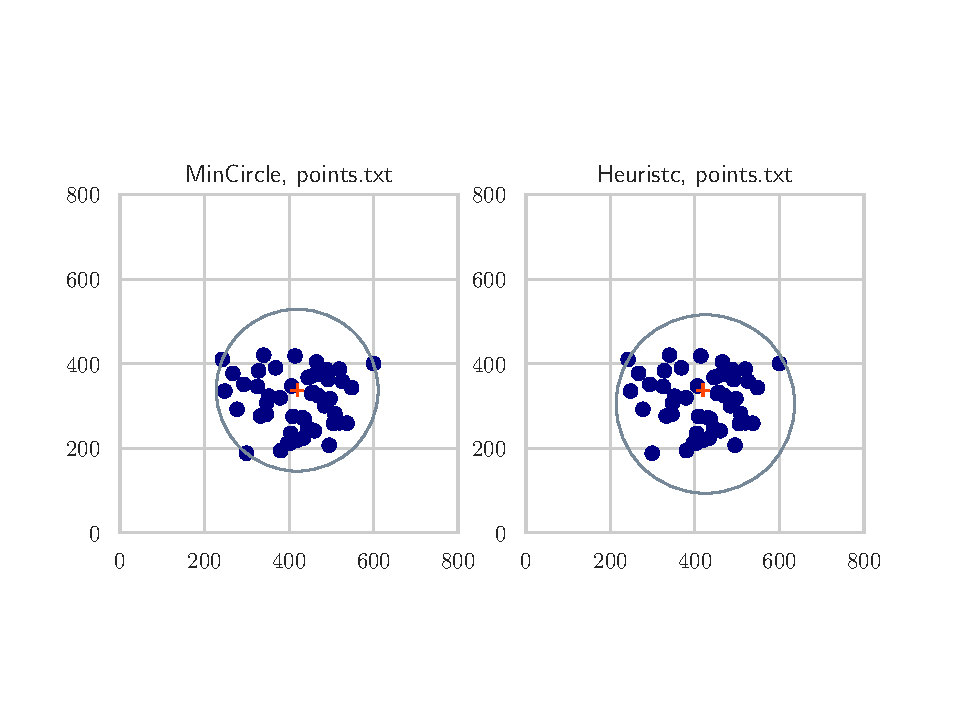
\includegraphics[scale=0.8]{figures/points/plot_min_circle.pdf}
\end{figure}


A seguir são apresentados os resultados considerando diferentes quantidades de pontos. Os experimentos consideraram 20, 200, 2000 e 20000 pontos para a implementação do círculo envolvendo utilizando os algoritmos de Círculo Mínimo e o algoritmo Heurístico.

Os resultados gráficos mostram que os algoritmos foram capazes de traçar o círculo mínimo de maneira satisfatória. Além disso, como esperado, o círculo mínimo possui resultados menos distorcidos do que o algoritmo heurístico (que é uma aproximação).

\begin{figure}[H]
  \centering
  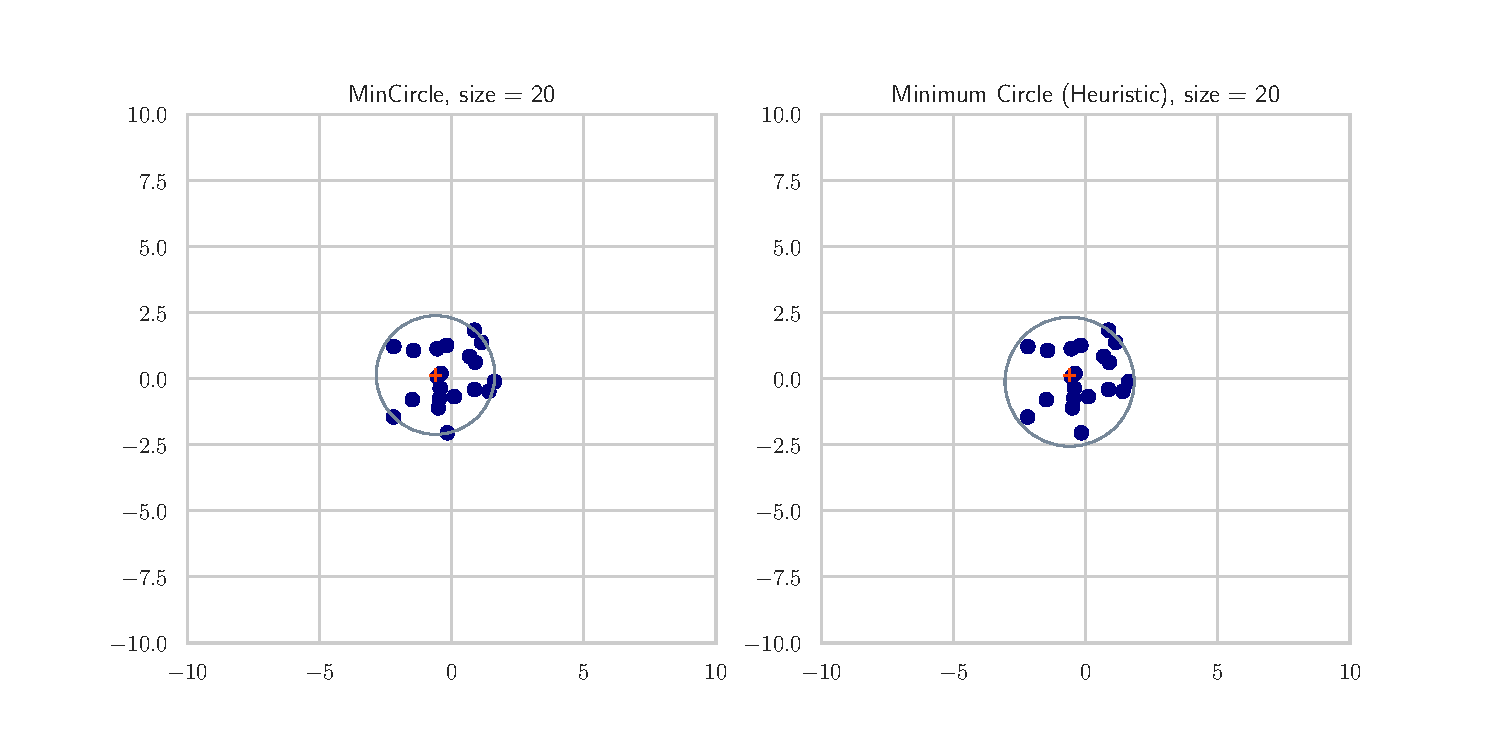
\includegraphics[scale=0.6]{figures/simulation/plot_min_circle_20_points.pdf}
\end{figure}

\begin{figure}[H]
  \centering
  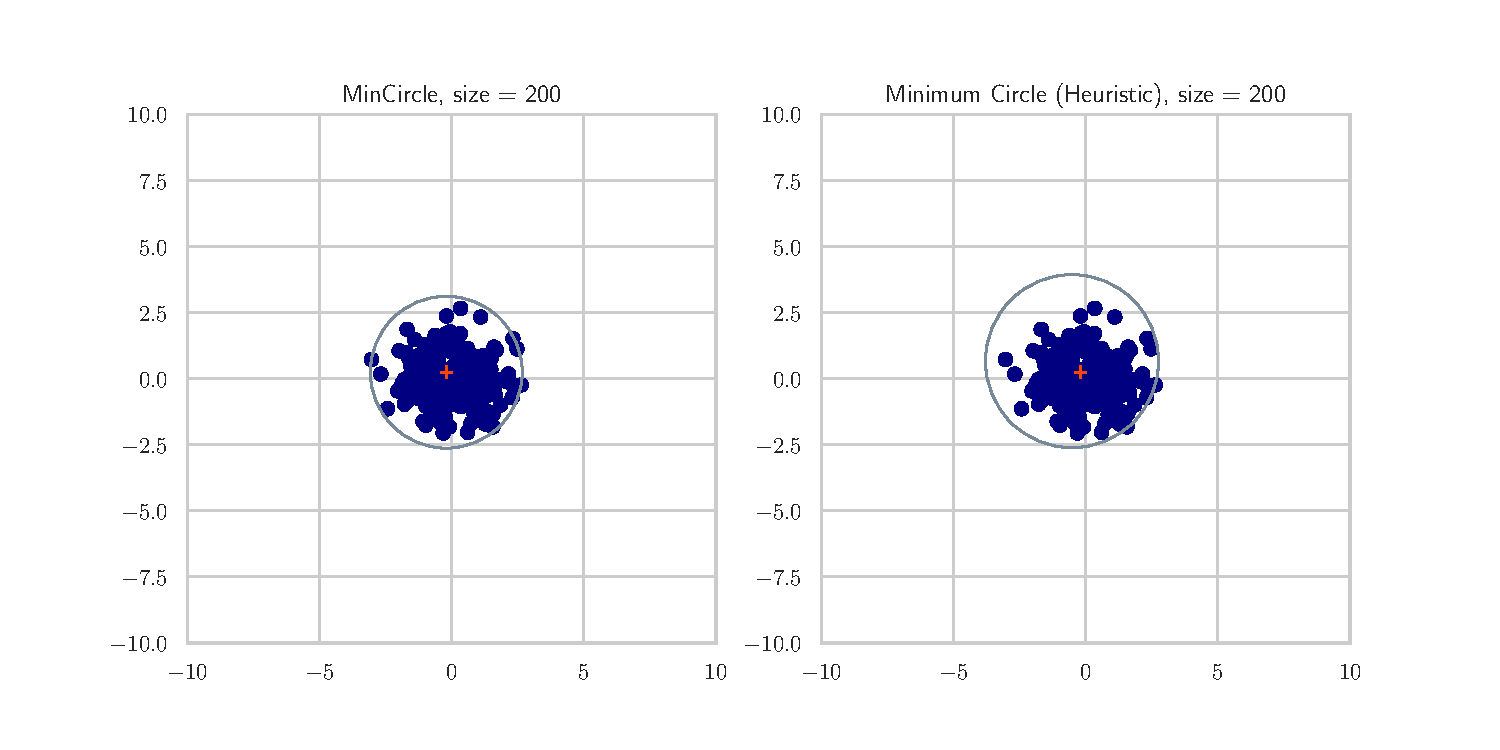
\includegraphics[scale=0.6]{figures/simulation/plot_min_circle_200_points.pdf}
\end{figure}

\begin{figure}[H]
  \centering
  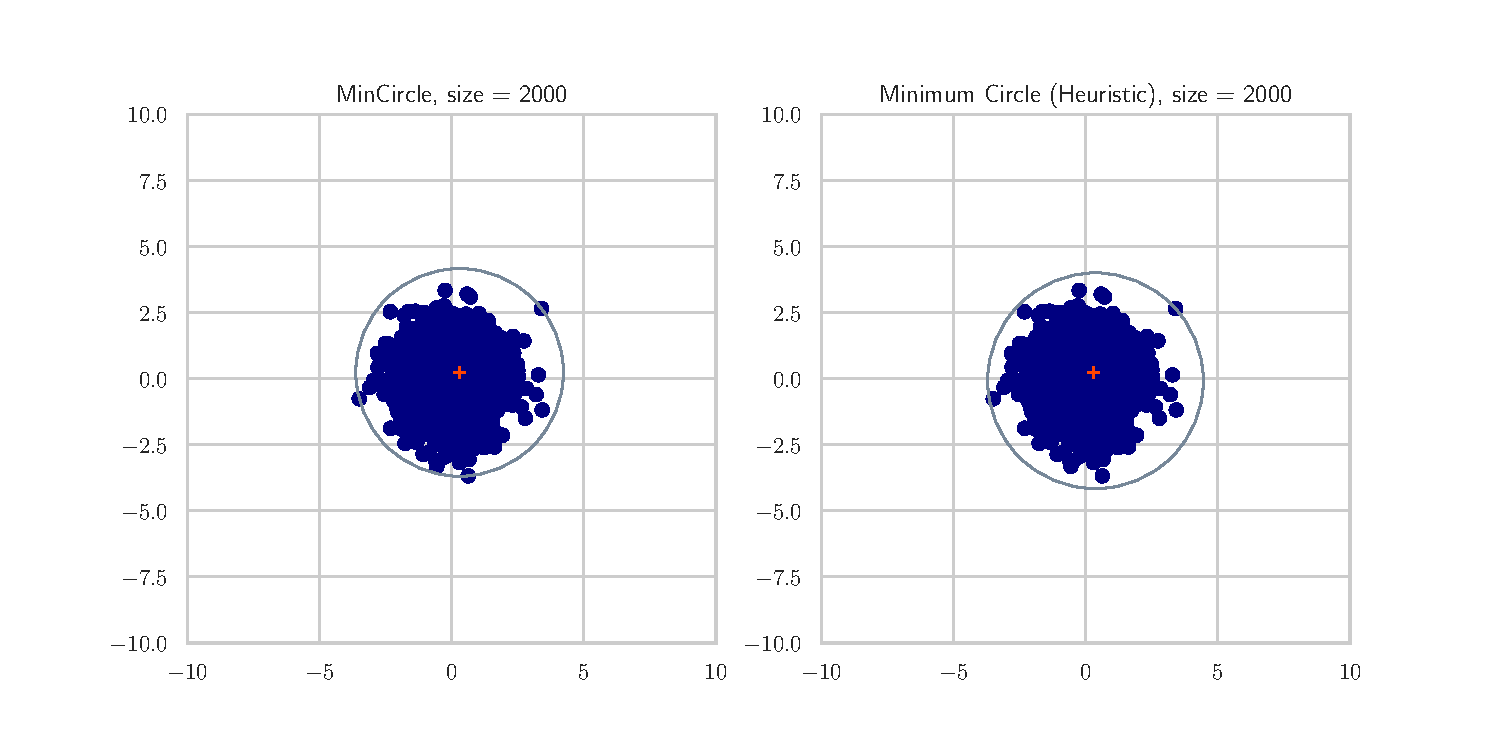
\includegraphics[scale=0.6]{figures/simulation/plot_min_circle_2000_points.pdf}
\end{figure}

\begin{figure}[H]
  \centering
  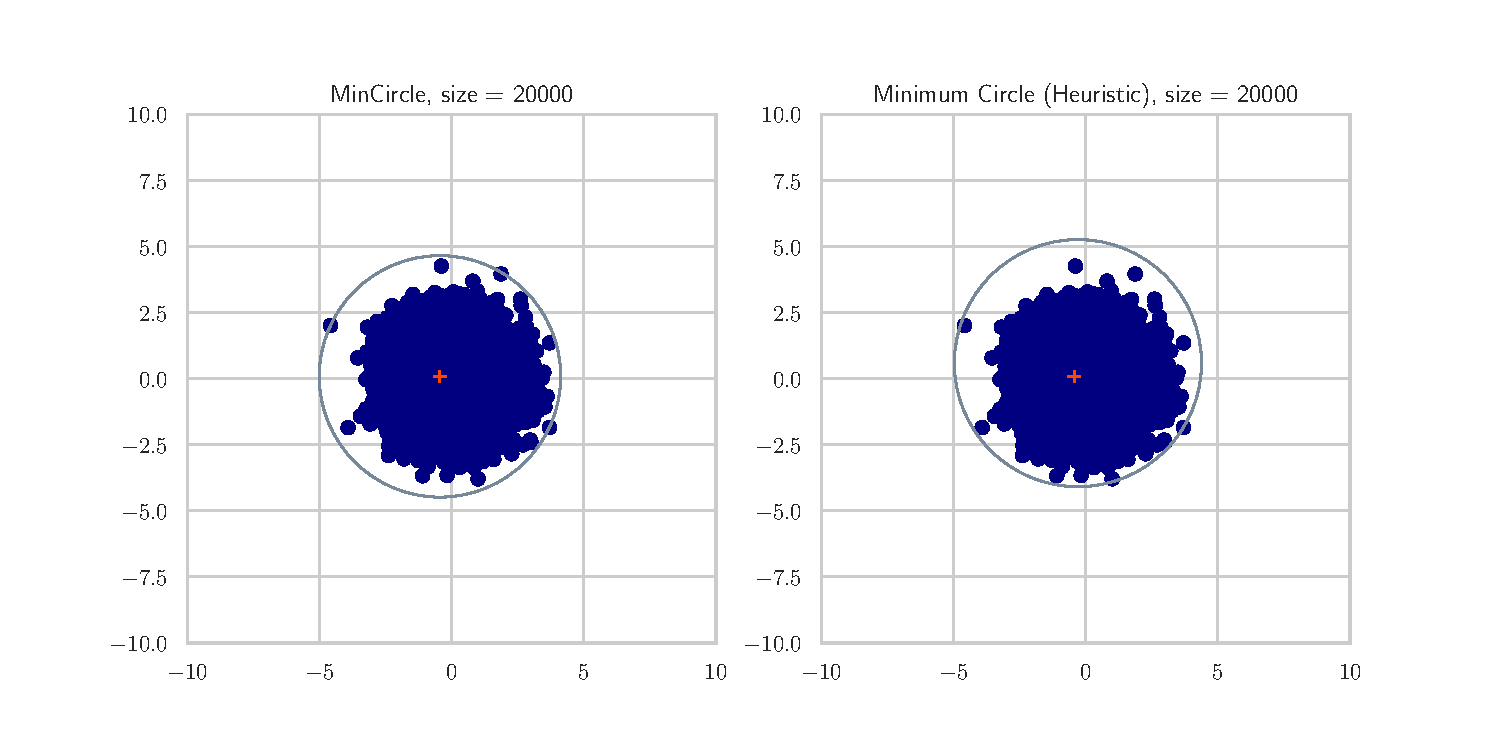
\includegraphics[scale=0.6]{figures/simulation/plot_min_circle_20000_points.pdf}
\end{figure}

Ao analisarmos o comportamento do tempo de execução dos algoritmos podemos notar que, assim como esperado, os algoritmos possuem um tempo de execução linear. Destaca-se que o algoritmo heurístico possui um tempo de execução para os dados simulados menor do que o algoritmo de círculo mínimo. 

\begin{figure}[H]
  \centering
  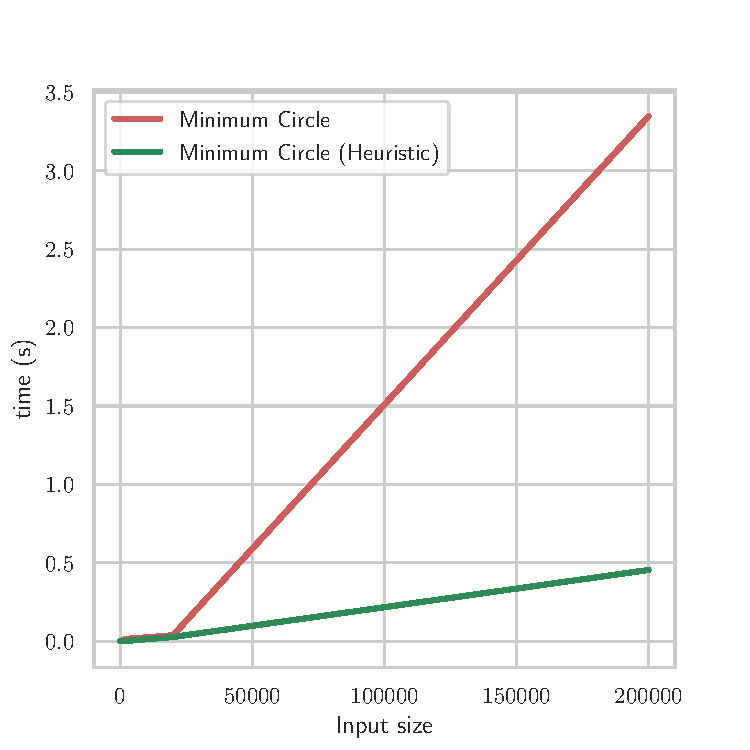
\includegraphics[scale=0.7]{figures/simulation/time.pdf}
\end{figure}

\section{Considerações finais}

Este trabalho apresentou a implementação do algoritmo heurístico e de círculo mínimo para definir o círculo envolvente em uma nuvem de pontos. Foram considerados dois experimentos. O primeiro com os dados que foram disponibilizados para a tarefa e o segundo a partir da geração de nuvem de pontos aleatórios.

Os resultados mostraram que os algortimos são eficientes, com destaque para o fato de que o algoritmo de círculo mínimo apresenta um resultado exato enquanto que o heurístico é uma aproximação do resultado. Além disso, foi observado que a partir dos experimentos realizados neste trabalho o algoritmo heurístico possui um tempo de execução linear (assim como o de círculo mínimo), porém melhor do que o algoritmo de círculo mínimo.

\end{document}